\documentclass[twocolumn,a4j]{jsarticle}
\setlength{\topmargin}{-18.5cm}
\setlength{\oddsidemargin}{-8.5mm}
\setlength{\evensidemargin}{-8.5mm}
\setlength{\textwidth}{19cm}
\setlength{\textheight}{26.5cm}

\usepackage[top=15truemm,bottom=20truemm,left=20truemm,right=20truemm]{geometry}
\usepackage[latin1]{inputenc}
\usepackage{amsmath}
\usepackage{amsfonts}
\usepackage{amssymb}
\usepackage[dvipdfmx]{graphicx}
\usepackage[hang,small,bf]{caption}
\usepackage[subrefformat=parens]{subcaption}
\usepackage[dvipdfmx]{color}
\usepackage{listings}
\usepackage{listings,jvlisting}
\usepackage{geometry}
\usepackage{framed}
\usepackage{color}
\usepackage[dvipdfmx]{hyperref}
\usepackage{ascmac}
\usepackage{enumerate}
\usepackage{tabularx}
\usepackage{cancel}
\usepackage{scalefnt}
\usepackage{overcite}
\usepackage{otf}
\usepackage{multicol}
\usepackage[geometry]{ifsym}

% キャプション後ろのダブルコロンを消す
\makeatletter
\long\def\@makecaption#1#2{%
  \vskip\abovecaptionskip
  \iftdir\sbox\@tempboxa{#1\hskip1zw#2}%
    \else\sbox\@tempboxa{#1 #2}%
  \fi
  \ifdim \wd\@tempboxa >\hsize
    \iftdir #1\hskip1zw#2\relax\par
      \else #1 #2\relax\par\fi
  \else
    \global \@minipagefalse
    \hbox to\hsize{\hfil\box\@tempboxa\hfil}%
  \fi
  \vskip\belowcaptionskip}
\makeatother

\renewcommand{\figurename}{Fig.}
\renewcommand{\tablename}{Table }

\makeatletter
\def\@maketitle
{
\begin{center}
{\LARGE \@title \par}
\end{center}
\begin{flushright}
{\large \@date}\\
{\large 京都工芸繊維大学 大学院 機械設計学専攻 計測システム工学研究室}\\
{\large M2 \@author}
\end{flushright}
\par\vskip 1.5em
}
\makeatother

\author{来代 勝胤 / KITADAI Masatsugu}
\title{令和5年度 11月度 共同研究報告書}
\date{2023/11/28}

\begin{document}
\columnseprule=0.1mm
\maketitle

\section*{報告内容}
\begin{enumerate}[1.]
	\item 三角翼後流の数値シミュレーションによる検証
\end{enumerate}

\section*{進捗報告}
今月は,計測手法の性能評価のための
数値シミュレーションデータの作成に取組み,
これまでの計測結果との比較を行った.

\section{三角翼後流の数値シミュレーションによる検証}
\subsection{乱流モデルの検討}
これまで計測したきた三角翼後流について,数値シミュレーションを用いた検証を行った.
解析を進める中で,乱流モデルの選択によって流れ場が大きく異なることがわかった.
今回の数値解析で使用したソフトウェアの詳細について以下の Table 1 に示す.
ここでは,計測結果との定性的な流れ場の検証を行うことを目的としているため,
時間間隔は 1/100 [s] とし,流れ場の十分な発展を考えて計算時間を 10 [s] とした.

\begin{table}[hbtp]
	\centering
	\caption{Condition of numerical simulation}
	\begin{tabular}{l c c}
		\hline
		Application     & OpenFOAM   & ver.10 \\ \hline
		Solver          & pimpleFoam          \\ \hline
		Time step       & 1/100      & s      \\ \hline
		Simulation time & 10         & s      \\ \hline
	\end{tabular}
\end{table}

また,乱流モデルの検証に用いた4つの条件を Table 2 に示す.
ここでは,Case 1 は乱流モデルを用いずに計算を行った場合であり,
Case 2,3 はRANSモデルの $k-\epsilon$ および $k-\omega$ SST を用いた場合,
Case 4 はLESモデルの Smagorinsky を用いた場合である.

\begin{table}[hbtp]
	\centering
	\caption{Turbulence Model}
	\begin{tabular}{l c c}
		\hline
		Case 1 &      & Laminar      \\ \hline
		Case 2 & RANS & $k-\epsilon$ \\ \hline
		Case 3 & RANS & $k-\omega$   \\ \hline
		Case 4 & LES  & Smagorinsky  \\ \hline
	\end{tabular}
\end{table}

\newpage
\subsection{数値解析モデル}
検証に用いる三角翼モデルを以下の Fig.1 に示す.
解析領域は実験で用いる回流水槽に基づいて決定しており,
主流方向は 代表長さ 120 [mm] の三角翼に対して,
10倍の長さとし,モデルの後端が $x=240$ [mm] に位置するように設定した.
また,このモデルの主流方向に対する迎角は 10 [deg] である.
\begin{figure}[htbp]
	\centering
	{
		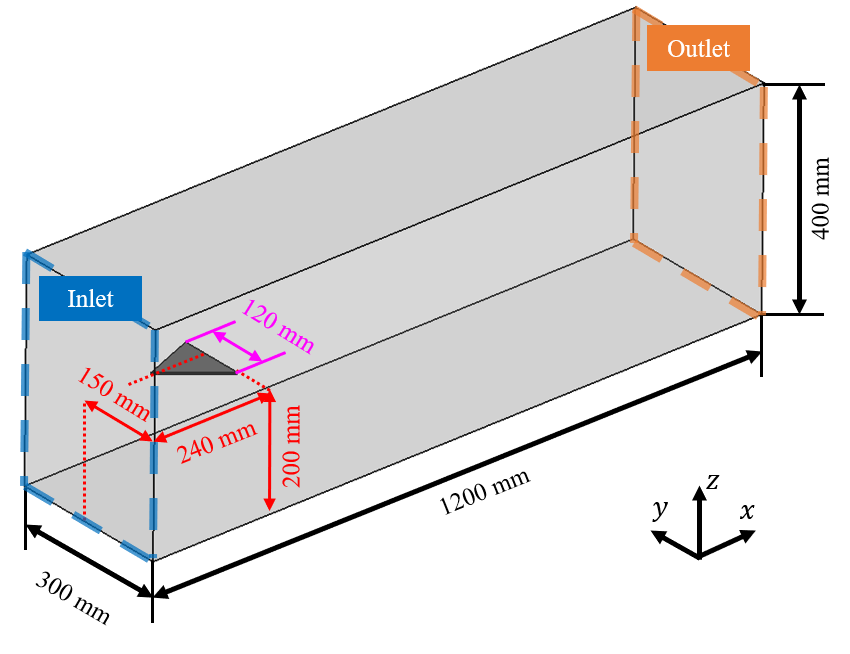
\includegraphics[keepaspectratio, width=70mm]{../images/Simulation/0_Mesh/Model_Birdseyeview.png}
		\subcaption{3D Model : Bird's-eye view}
		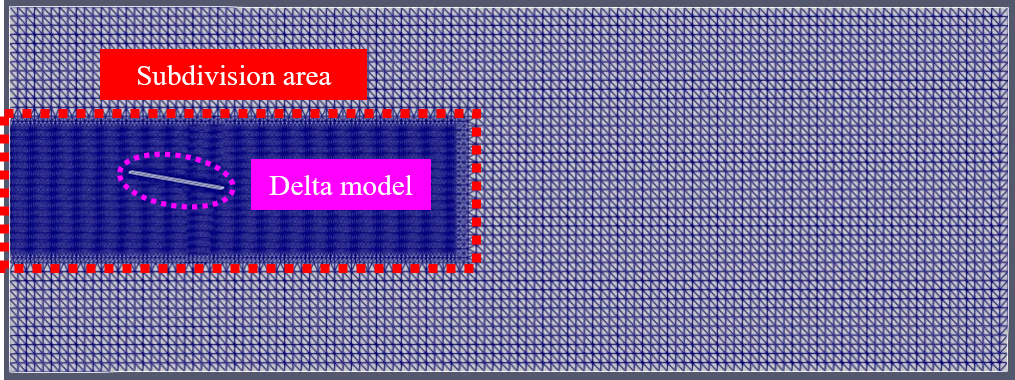
\includegraphics[keepaspectratio, width=65mm]{../images/Simulation/0_Mesh/Mesh_Sideview.png}
		\subcaption{Mesh : Side view}
	}
	\caption{Delta wing model}
\end{figure}

境界条件は,主流方向速度 $u = 250$ [mm/s] を初期条件として設定した.
その他の条件については,以下の Table 3 に示す.
また,流体の動粘性係数 $\nu$ を標準状態の水,代表長さ $L$ を三角翼の翼幅,
代表速度 $U$ を主流方向速度としてレイノルズ数を計算すると
$\rm{Re} = 3.0 \times 10^{4}$ となる.

\begin{table}[hbtp]
	\centering
	\caption{Boundary conditions}
	\begin{tabular}{l c c}
		\hline
		       & $U$ [m/s]     & $P$ [Pa]      \\ \hline
		Inlet  & (0.25, 0, 0)  & Zero Gradient \\ \hline
		Outlet & Zero Gradient & 0             \\ \hline
		Others & Slip          & Zero Gradient \\ \hline
	\end{tabular}
\end{table}

\newpage
\subsection{数値解析結果}
それぞれの条件で数値計算を行い,その結果を比較する.
まず,各条件について計算に要した時間を以下の Fig.2 に示す.
最も早く計算が終了したのは Case 4 : LES (Smagorinsky) モデル であり,
次いで Case 1 : Laminar モデル である.
一方で,Case 2,3 の RANS モデル は計算時間が長くなっており,
Case 1,4 に比べて 10 \% 以上の時間を要することがわかる.
\begin{figure}[htbp]
	\centering
	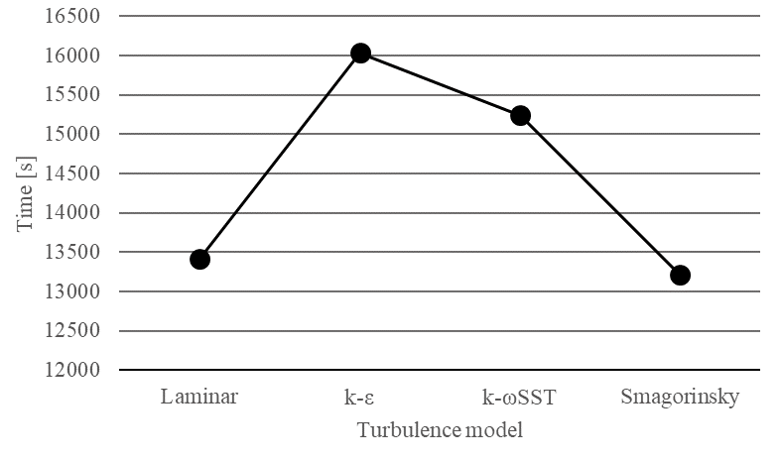
\includegraphics[keepaspectratio, width=80mm]{../images/Simulation/Time_for_Numerical_Simulation.png}
	\caption{Time required for numerical simulation}
\end{figure}

次に,実際に計算された流れ場を確認する.
今回は,翼後端を $x=0$ として,$x=0, 20, 40$ [mm] の位置を比較対象とする.
ここで,(b) に示す図はメッシュセルの位置を示しており,
この位置の速度情報を用いて速度場を取得する.
\begin{figure}[htbp]
	\centering
	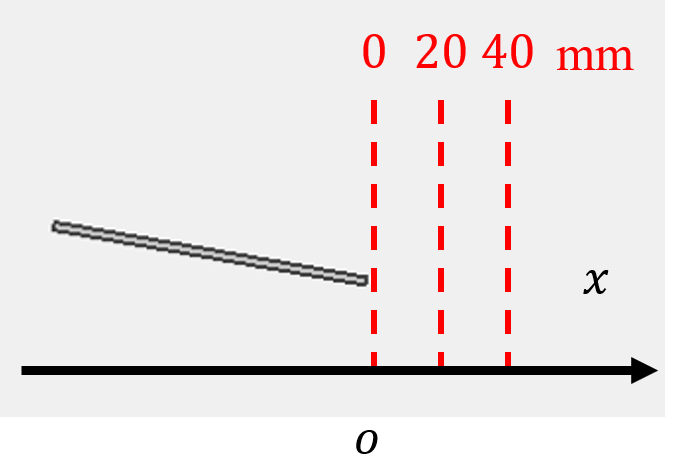
\includegraphics[keepaspectratio, width=60mm]{../images/Simulation/Schematic_Delta-Wing.png}
	\caption{Schematic of delta wing}
\end{figure}

結果をみると,Case 1,3,4 は同じような流れ場を示し,
(a) の実験結果とも定性的に一致している箇所も見受けられる.
しかし,$k-\epsilon$ モデルを利用した Case 2 は,
他の条件とは大きく異なる流れ場を示していることがわかる.

\section{12月の予定}
\begin{itemize}
	\item 数値シミュレーションを用いた計測性能評価
	\item 車両モデルの計測
	\item 論文の作成
\end{itemize}

\newpage
\begin{figure}[htbp]
	\subsubsection*{$\blacksquare$ $x=0$ [mm]}
	\centering
	{
		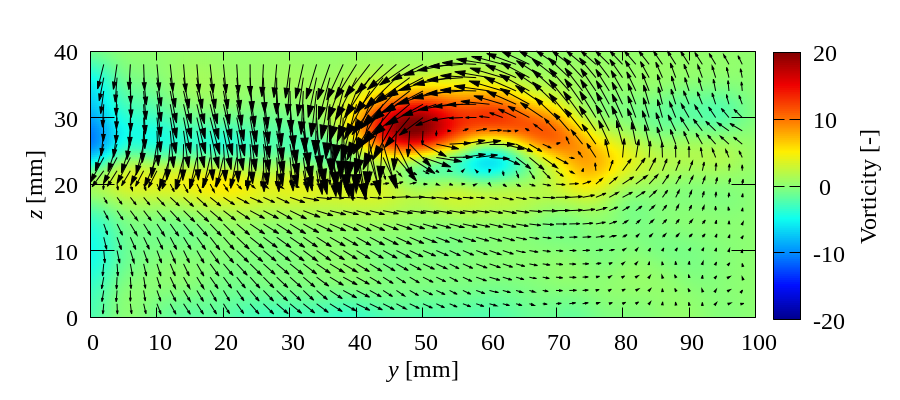
\includegraphics[keepaspectratio, width=78mm]{../images/Simulation/Compare/experiment_x=0.png}
		\subcaption{Experiment}
		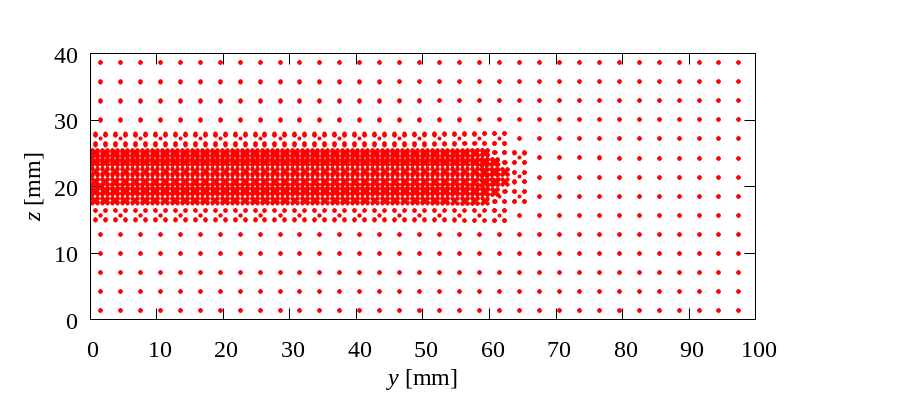
\includegraphics[keepaspectratio, width=78mm]{../images/Simulation/0_Mesh/x=0.png}
		\subcaption{Grid point of cell}
		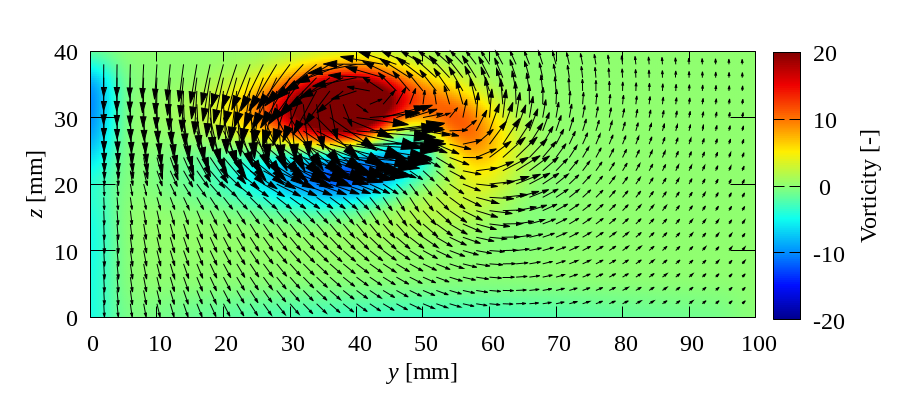
\includegraphics[keepaspectratio, width=78mm]{../images/Simulation/1_Laminar/x=0.png}
		\subcaption{Case 1 : Laminar}
		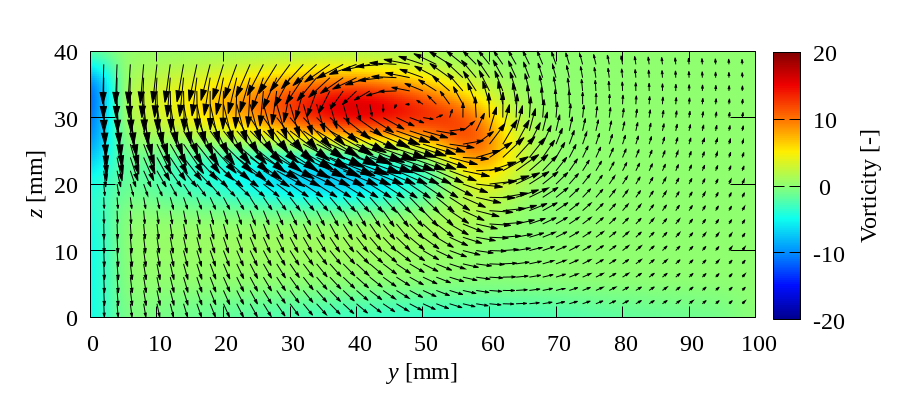
\includegraphics[keepaspectratio, width=78mm]{../images/Simulation/2_kEpsilon/x=0.png}
		\subcaption{Case 2 : RANS ($k-\epsilon$)}
		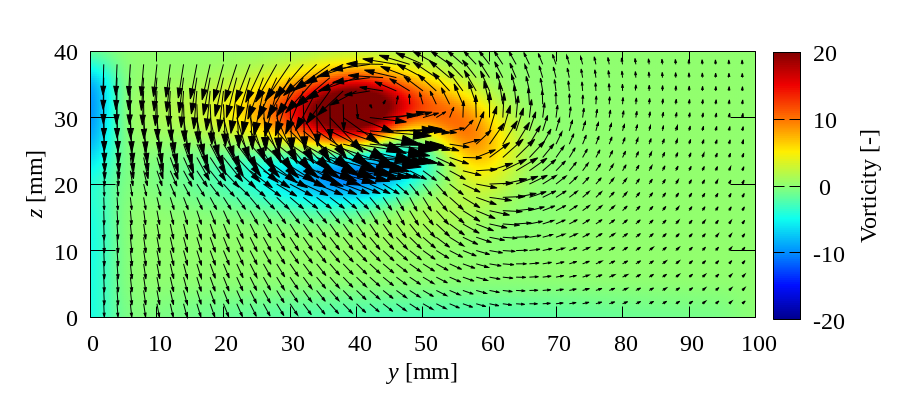
\includegraphics[keepaspectratio, width=78mm]{../images/Simulation/3_kOmegaSST/x=0.png}
		\subcaption{Case 3 : RANS ($k-\omega$ SST)}
		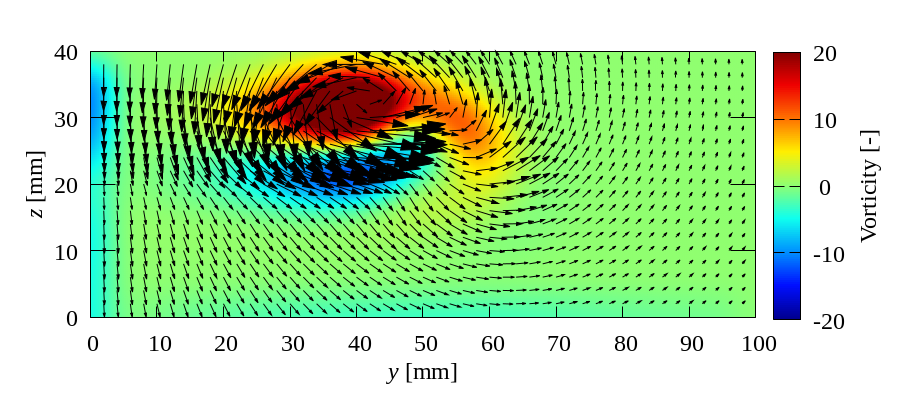
\includegraphics[keepaspectratio, width=78mm]{../images/Simulation/4_Smagorinsky/x=0.png}
		\subcaption{Case 4 : LES (Smagorinsky)}
	}
	\caption{Delta wing :$x=0$}
\end{figure}

\newpage
\begin{figure}[htbp]
	\subsubsection*{$\blacksquare$ $x=20$ [mm]}
	\centering
	{
		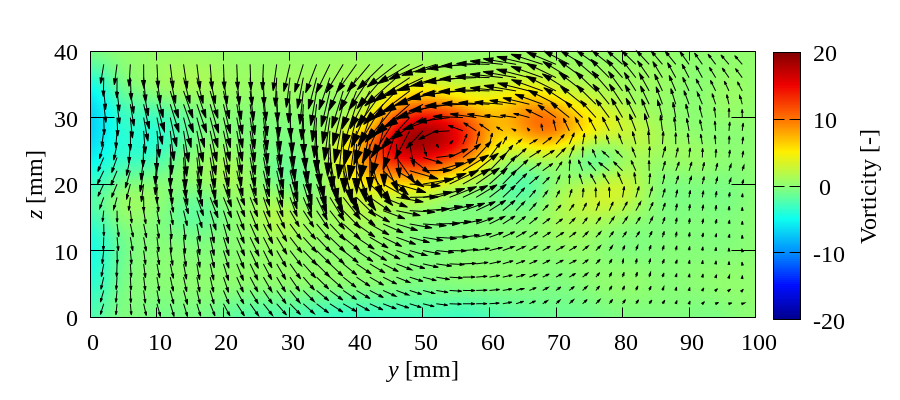
\includegraphics[keepaspectratio, width=78mm]{../images/Simulation/Compare/experiment_x=20.png}
		\subcaption{Experiment}
		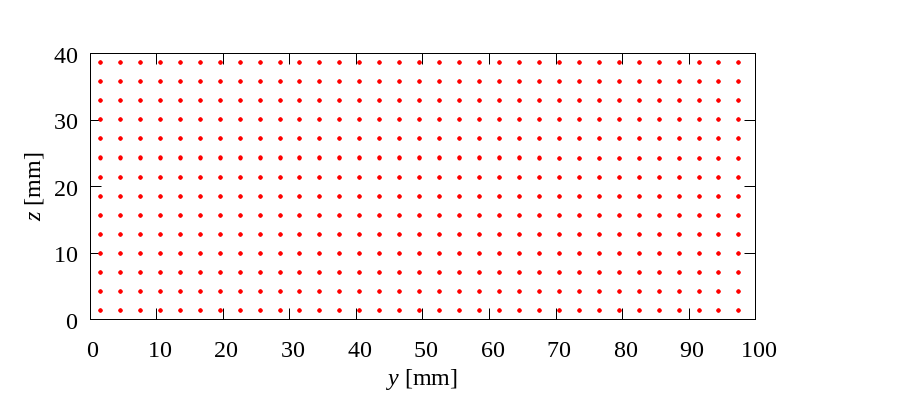
\includegraphics[keepaspectratio, width=78mm]{../images/Simulation/0_Mesh/x=20.png}
		\subcaption{Grid point of cell}
		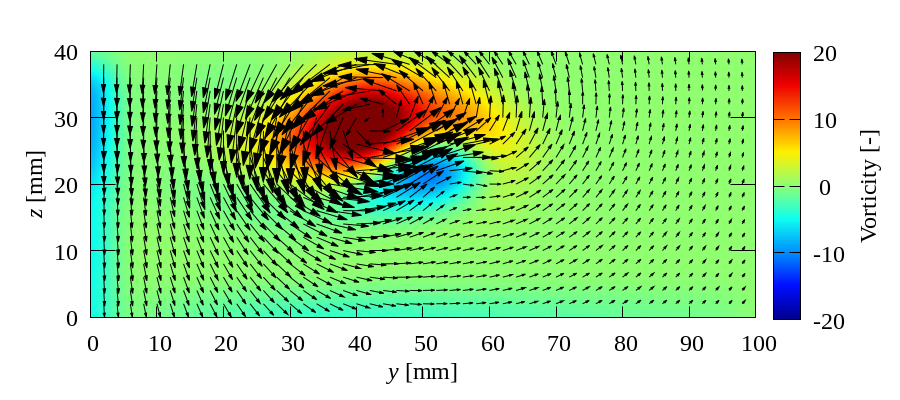
\includegraphics[keepaspectratio, width=78mm]{../images/Simulation/1_Laminar/x=20.png}
		\subcaption{Case 1 : Laminar}
		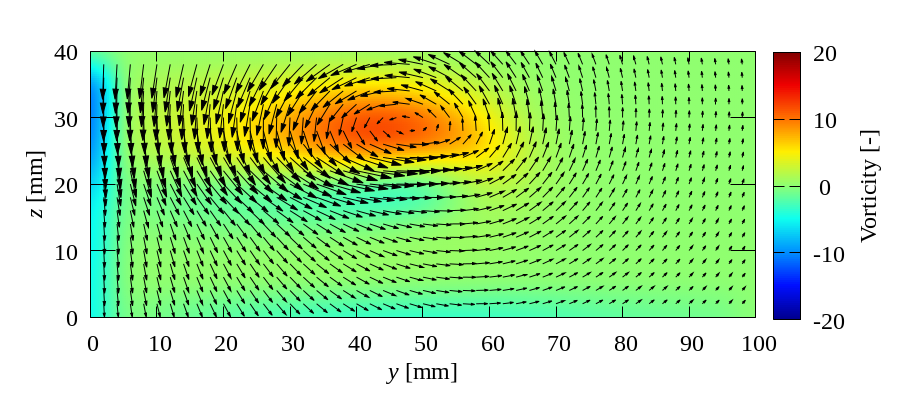
\includegraphics[keepaspectratio, width=78mm]{../images/Simulation/2_kEpsilon/x=20.png}
		\subcaption{Case 2 : RANS ($k-\epsilon$)}
		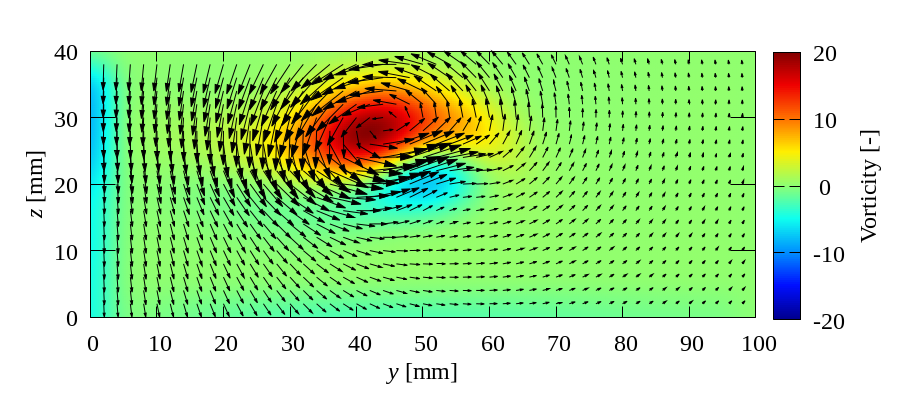
\includegraphics[keepaspectratio, width=78mm]{../images/Simulation/3_kOmegaSST/x=20.png}
		\subcaption{Case 3 : RANS ($k-\omega$ SST)}
		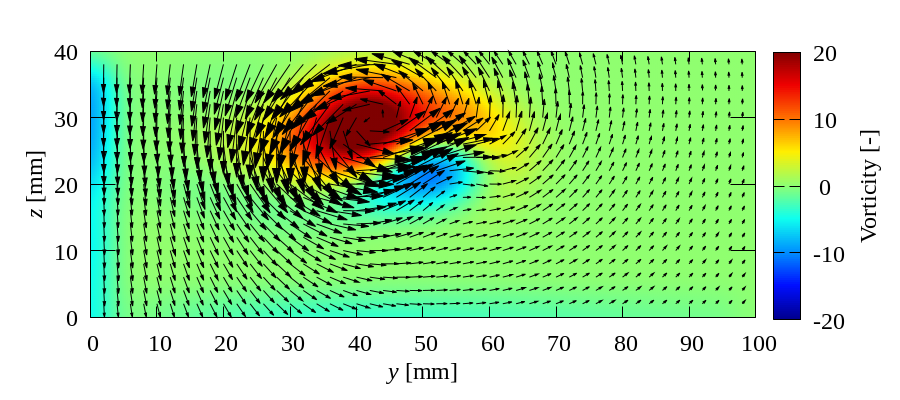
\includegraphics[keepaspectratio, width=78mm]{../images/Simulation/4_Smagorinsky/x=20.png}
		\subcaption{Case 4 : LES (Smagorinsky)}
	}
	\caption{Delta wing :$x=20$}
\end{figure}

\newpage
\begin{figure}[htbp]
	\subsubsection*{$\blacksquare$ $x=40$ [mm]}
	\centering
	{
		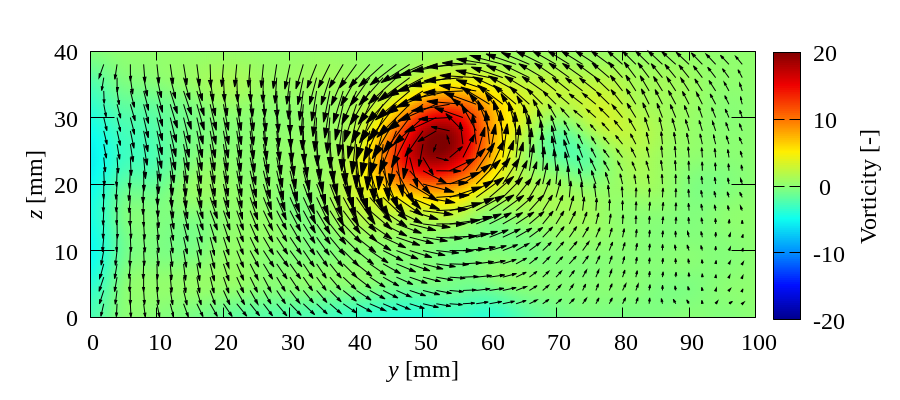
\includegraphics[keepaspectratio, width=78mm]{../images/Simulation/Compare/experiment_x=40.png}
		\subcaption{Experiment}
		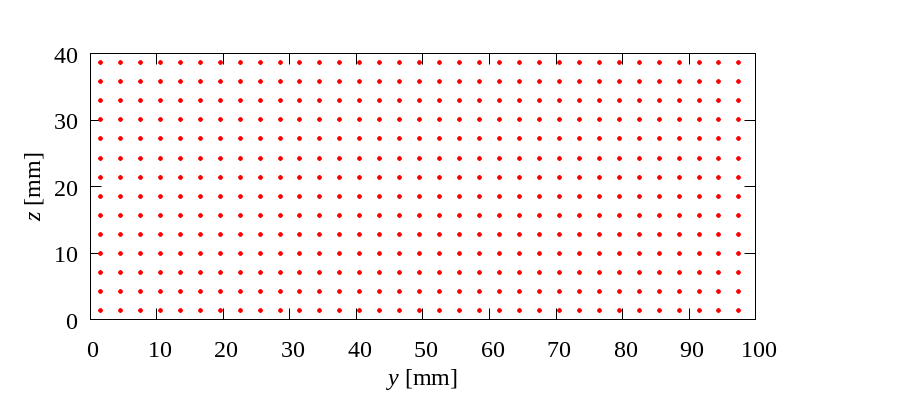
\includegraphics[keepaspectratio, width=78mm]{../images/Simulation/0_Mesh/x=40.png}
		\subcaption{Grid point of cell}
		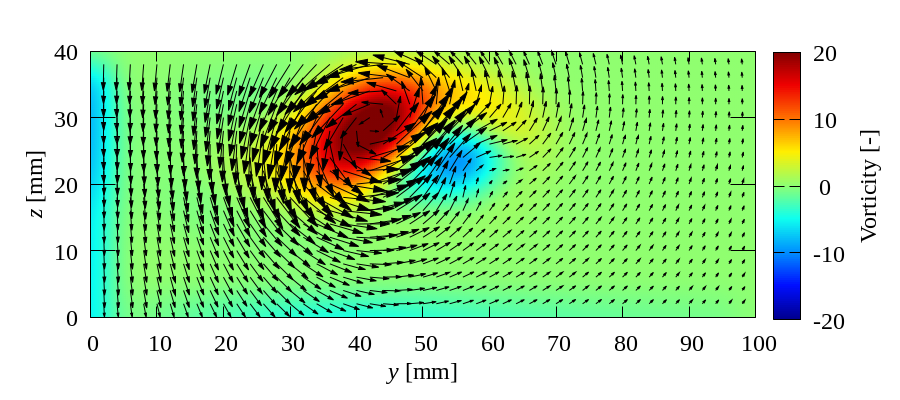
\includegraphics[keepaspectratio, width=78mm]{../images/Simulation/1_Laminar/x=40.png}
		\subcaption{Case 1 : Laminar}
		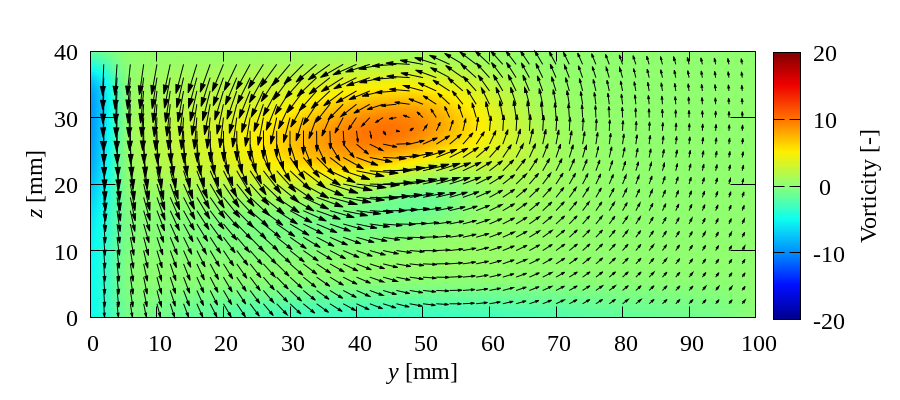
\includegraphics[keepaspectratio, width=78mm]{../images/Simulation/2_kEpsilon/x=40.png}
		\subcaption{Case 2 : RANS ($k-\epsilon$)}
		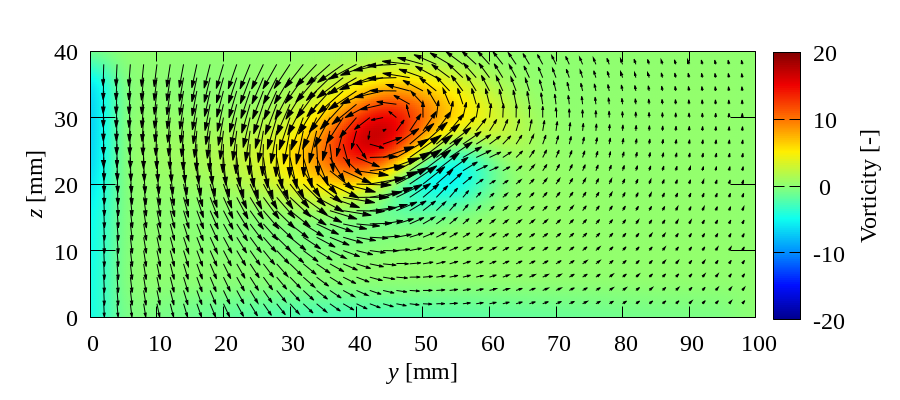
\includegraphics[keepaspectratio, width=78mm]{../images/Simulation/3_kOmegaSST/x=40.png}
		\subcaption{Case 3 : RANS ($k-\omega$ SST)}
		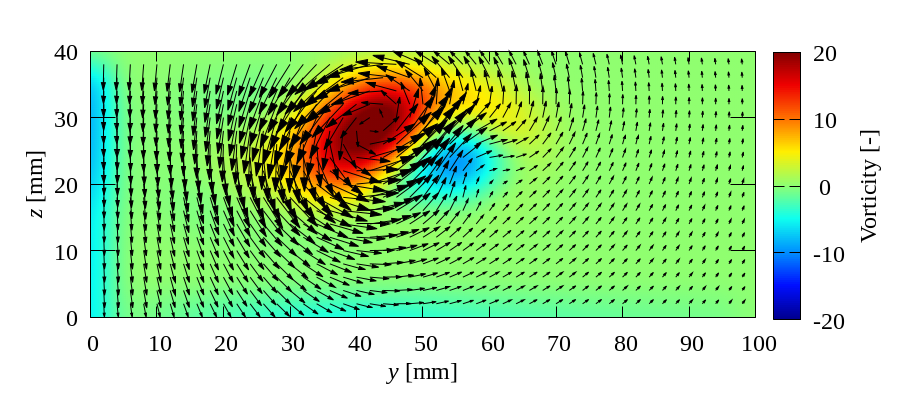
\includegraphics[keepaspectratio, width=78mm]{../images/Simulation/4_Smagorinsky/x=40.png}
		\subcaption{Case 4 : LES (Smagorinsky)}
	}
	\caption{Delta wing :$x=40$}
\end{figure}

\end{document}